\documentclass[12pt,a4paper]{article}
\usepackage{ucs}
\usepackage{caption}
\usepackage[latin1,utf8x]{inputenc}
\usepackage{amsmath}
\usepackage{caption}
\captionsetup{font=small,labelfont=bf}
\usepackage[danish]{babel}
\usepackage[rmargin=3cm,tmargin=3.3cm]{geometry}
\usepackage{listings}
\usepackage{color}
\setlength{\parindent}{0pt}
\setlength{\parskip}{1ex plus 0.5ex minus 0.2ex}
\usepackage{graphicx}
\usepackage{fixltx2e}


%insert links
\usepackage{hyperref}
\usepackage{fancyhdr,lastpage}	
\pagestyle{fancy}


\definecolor{mygreen}{rgb}{0,0.6,0}
\definecolor{myblue}{rgb}{0,0,1}
\definecolor{myyellow}{rgb}{0.7,0.7,0}
\definecolor{myblack}{rgb}{0,0,0}

\lstset{
	breaklines=true,
	numbers=left, 
	commentstyle=\color{mygreen},
	stringstyle=\color{myyellow},
}

%header
\lhead{ 
	Embedded Systems \\
	02131 \\ 
}
\chead{ 
}
\rhead{ 2 October, 2012 \\ \bigskip  }

%Footer
\lfoot{
	\rule{\textwidth}{0.1mm}\\
}

\cfoot{}
\rfoot{\ \\ \scriptsize{Side \thepage\ af \pageref{LastPage}}}

\begin{document}

%Forside
\begin{titlepage}
	\begin{center}
		\vspace*{13\baselineskip}
		\huge
		\bfseries
		Embedded Systems\\ 
		\ \\
		02131 \\[5\baselineskip]

		\normalfont
		\Large
		R-peak detection!\\	
		2013

		\small
		\vfill
	\end{center}	
	\begin{flushleft}
		Jakob Welner, s124305\\
	 	Jacob Gjerstruo, s113440\\
	\end{flushleft}
\end{titlepage}

\ \\
\section*{Abstract}


\thispagestyle{empty} 
\newpage

%Table of Contents
\tableofcontents
\thispagestyle{empty} 
\newpage

%Reset pagecount
\setcounter{page}{1}

%Alm. sider
\ \\
\section{Introduction}
	
\subsection{Requirements}
Below follows a list of functional and non-functional requirements:\\

\textbf{ Functional requirements for the application:}
\begin{itemize}
	\item Data acquisition in simulated real-time (Discrete data)
	\item Implementation of the 5 filters
	\item Implementation of the R-peak detection
	\item Output of relevant data to the user, based on the algorithm
	\item An analysis of our implementation as well as the critical parts, runtime and memory requirements.
\end{itemize}
\textbf{Non-functional requirements for the application:}
\begin {itemize}
	\item Using the C-programming language for software development
\end{itemize}

\section{Theory}
 	In order to initiate the structure- and design-process of the program, a number of questions needed to be answered first:\\
 	
 	\begin{enumerate}
	\item How should the real-time data acquisition be simulated?
	\item How should the filters be integrated?
	\item How should the R-peak detection be integrated?
	\item Which data would be relevant for the user, and how should it be shown?
	\item How do you determine the critical parts of the software?
\end{enumerate}

\subsection{Problem 1: Data acquisition}
	
\subsection{Problem 2: Implementation of Filters}
	
\subsection{Problem 3: Implementation of R-peak detection}

\subsection{Problem 4: Relevant data}

\subsection{Problem 5: Critical parts}

\section{Design}

\section{Implementation}
\subsection{Core structure}

\subsection{Real-time data acquisition}

\subsection{Implementation of Filters}
	
\subsection{Implementation of RPeakDetection}
	
\subsection{Relevant data}
	
\subsection{Critical parts}

\section{Results}
	
%	\begin{figure}[h!]
%		\centering
%			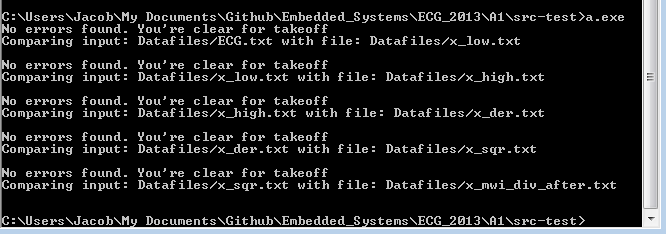
\includegraphics[width=1\textwidth]{Screenshots/tests_filter_result.png}
%		\caption{A screenshot of the output of the tests of the filters.}
%		\label{test_filter_result}
%	\end{figure}

\section{Discussion}
	
\subsection{Improvements}

\section{Conclusion}
\newpage
\begin{thebibliography}{9}

\bibitem{lamport94}
  Michael Reibel Boesen, Jan Madsen, Linas Kaminskas, Paul Pop, Karsten Juul Frederiksen\\
  \emph{Assignment 2: The ECG processor}\\
  2013.\\

\bibitem{Gezel}
  \emph{Lecture7: Finite state machine with Datapath}\\
  Fall, 2007.\\

\bibitem{GezelBasicSyntax}
  \emph{GEZEL Basic Syntax}\\
\end{thebibliography}
	
\newpage	
	\begin{Large}
		\textbf{Appendix}
	\end{Large}
	\appendix

\section{Who wrote what}
Jacob Gjerstrup, s113440 wrote: \\
Jakob Welner, s124305 wrote: \\

\section{Output of the RPeakDetection}
	
\section{Sourcecode - introductionary exercises}
	
\section{Sourcecode - the real program}

\subsection{Buffer}
	%\lstinputlisting[language=C]{Code/buffer.c}	
\subsection{Filters}
\subsection{RPeakDetection}
\subsection{Sensor}
\subsection{Header files}
\subsubsection{sensor.h}
\subsubsection{buffer.h}
\subsection{Tests}
\end{document}